\documentclass[11pt]{article}

\oddsidemargin=0in
\evensidemargin=0in
\textwidth=6.3in
\topmargin=-0.5in
\textheight=9in

\parindent=0in
%\pagestyle{empty}

\usepackage{graphicx}
\usepackage[english]{babel}
\usepackage[latin1]{inputenc}
\usepackage{times}
\usepackage[T1]{fontenc}
\usepackage{amsmath}
\usepackage{amssymb}
\usepackage{subfigure}
\usepackage{algorithmic}
\usepackage{algorithm}
\usepackage{url}


\newcommand{\argmax}{\mathop{\arg\max}}
\newcommand{\deriv}[2]{\frac{\partial{#1}}{\partial {#2}} }
\newcommand{\dsep}{\mbox{dsep}}
\newcommand{\Pa}{\mathop{Pa}}
\newcommand{\ND}{\mbox{ND}}
\newcommand{\De}{\mbox{De}}
\newcommand{\Ch}{\mbox{Ch}}
\newcommand{\graphG}{{\mathcal{G}}}
\newcommand{\graphH}{{\mathcal{H}}}
\newcommand{\setA}{\mathcal{A}}
\newcommand{\setB}{\mathcal{B}}
\newcommand{\setS}{\mathcal{S}}
\newcommand{\setV}{\mathcal{V}}
\DeclareMathOperator*{\union}{\bigcup}
\DeclareMathOperator*{\intersection}{\bigcap}
\DeclareMathOperator*{\Val}{Val}
\newcommand{\mbf}[1]{{\mathbf{#1}}}
\newcommand{\eq}{\!=\!}
\newcommand{\cut}[1]{{}}

\begin{document}

%%%(change to appropriate class and semester)
{\centering
  \rule{6.3in}{2pt}
  \vspace{1em}
  \Large{Notes on RBM Learning\\}
  Benjamin M. Marlin\\
  \vspace{0.1em}
  \rule{6.3in}{1.5pt}
}
\vspace{1pc}

\section{Introduction}
The binary restricted Boltzmann machine (RBM) model is a Markov network model with two layers of variables $\mbf{X}$ and $\mbf{H}$. The $\mbf{X}$ variables $X_1,...,X_D$ constitute the first layer of the model and are referred to as the \textit{visible variables} or \textit{visible units}. The second layer of the model consists of the $\mbf{H}$ variables $H_1,...,H_K$ referred to as the \textit{hidden variables} or \textit{hidden units}. The Markov network structure underlying the RBM is a bipartite graph where there are edges between the visible units and the hidden units, but not within the hidden units or within the visible units. 
The classical version of the model uses all binary variables.\\

\begin{figure}[ht]
\centering
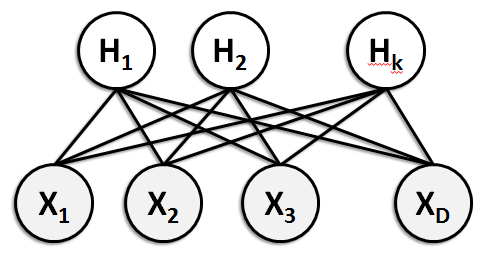
\includegraphics[width=2.5in]{Figures/rbm.png}
\caption{RBM Graphical Model}
\end{figure}

In the context of learning models for binary images, the $\mbf{X}$ variables represent the binary pixels of the image. It is more convenient to consider each image as a vector of length $D$ for use with this model. The hidden units are also a binary vector of length $K$. When $K$ is less than $D$, we can view the hidden units as a lower-dimensional encoding of the image. We can think of learning the RBM model parameters roughly as learning to extract features that can be used to encode the visible units with minimal loss of information. This encoding can be used for a variety of tasks including classification and information retrieval.\\

\section{Probabilistic Model} The probabilistic model underlying the RBM is essentially the same as that underlying the Ising model and the CRF model. The main difference is that in the RBM, the hidden variables are never observed. The model can be defined through a joint energy function on the hidden and visible variables as seen below. The model parameters $W^P_{dk}$ encode the
pairwise compatibility between $x_d$ and $h_k$. The model parameters $W^B_k$ and $W^C_d$
provide a bias that either encourages or discourages $h_k$ and $x_d$ from turning on.

\begin{align}
\label{energy}
E_W(\mbf{x},\mbf{h})&=
-\sum_{d=1}^D\sum_{k=1}^K W^P_{dk}x_dh_k - \sum_{k=1}^KW^B_k h_k - \sum_{d=1}^D W^C_d x_d
\end{align}

Using the standard log-linear mapping between energies and probabilities, we obtain the joint distribution over the visible and hidden variables as follows. Like the Ising model and CRF, the partition function of the RBM is a sum over all configurations of all the variables in the model.

\begin{align}
\label{joint-prob}
P_W(\mbf{X}=\mbf{x},\mbf{H}=\mbf{h})&= \frac{\exp(-E_W(\mbf{x},\mbf{h}))}
{\sum_{\mbf{x}'}\sum_{\mbf{h}'}\exp(-E_W(\mbf{x}',\mbf{h}'))}
\end{align}

Since the hidden variables are never observed, when we learn the model parameters we must marginalize away the hidden variables and optimize the log likelihood of the parameters given the values of the visible variables only. The marginal probability of the visible variables is given below.

\begin{align}
\label{marginal-prob}
P_W(\mbf{X}=\mbf{x})&= \sum_{\mbf{h}}P_W(\mbf{X}=\mbf{x},\mbf{H}=\mbf{h}) \\
&=\frac{\sum_{\mbf{h}}\exp(-E_W(\mbf{x},\mbf{h}))}
{\sum_{\mbf{x}'}\sum_{\mbf{h}'}\exp(-E_W(\mbf{x}',\mbf{h}'))}
\end{align}


\section{Inference} One of the main benefits of RBM models relative to other models is that inference for the visible variables given the hidden variables and inference for the hidden variables given the visible variables is very easy due to the structure of the graph. In particular, given all of the $\mbf{X}$ variables, all of the $\mbf{H}$ variables are independent of each other since there are no connections within the hidden layer. By symmetry, the $\mbf{X}$ variables are all independent of each other given the $\mbf{H}$ variables. This gives us a very simple block-Gibbs algorithm for drawing samples from an RBM. The algorithm alternates between sampling each visible unit independently of the other visible units conditioned on all of the hidden units and sampling each hidden unit independently of the other hidden units given the values for the visible units. The required conditional probabilities are given below.

\begin{align}
\label{pxgh}
P_W(X_d=x_d|\mbf{h})&= \frac{\exp(W^C_dx_d + \sum_{k=1}^K W^P_{dk}x_dh_k)}
{1+ \exp(W^C_d + \sum_{k=1}^K W^P_{dk}h_k) }\\
\label{phgx}
P_W(H_k=h_k|\mbf{x})&= \frac{\exp(W^B_kh_k + \sum_{d=1}^D W^P_{dk}x_dh_k )}
{1+ \exp(W^B_k + \sum_{d=1}^D W^P_{dk}x_d + ) }
\end{align}

The complete block Gibbs sampling algorithm for the RBM is listed below. Recall that to draw a sample $z$ from a distribution $P(Z)$ over a binary random variable $Z$, we first draw a random number $u$ from a uniform distribution on $[0,1]$. We set $z=1$ if $u<P(Z=1)$ and $z=0$ otherwise. Combined with the conditional distributions listed above, this is all you need to implement the block Gibbs sampler given RBM parameters $W^P$,$W^B$ and $W^C$.\\

\begin{algorithm}[h!]
\begin{algorithmic}
\STATE $RBMBlockGibbsSample(W^P,W^B,W^C,S)$
\STATE \textbf{for} $k$ from $1$ to $K$ Initialize $h_k^0$ to a random binary value
\FOR{$s$ from $1$ to $S$}
\STATE $\mbf{x}^s \leftarrow \mbox{gibbs\_x\_step}(\mbf{h}^{s-1},W^P,W^C)$
\STATE $\mbf{h}^s \leftarrow \mbox{gibbs\_h\_step}(\mbf{x}^{s},W^P,W^B)$
\ENDFOR
\STATE Return $\mbf{x}^1,...,\mbf{x}^S$ and $\mbf{h}^1,...,\mbf{h}^S$
\end{algorithmic}
\caption{Block Gibbs Sampler for the RBM model}
\label{inference}
\end{algorithm}

\begin{algorithm}[h!]
\begin{algorithmic}
\STATE $\mbox{gibbs\_x\_step}(\mbf{h},W^P,W^C)$
\STATE \textbf{for} $d$ from $1$ to $D$: Sample $x_d \sim P_W(X_d|\mbf{h})$
\STATE Return $\mbf{x}$
\end{algorithmic}
\caption{Gibbs X Step}
\end{algorithm}

\begin{algorithm}[h!]
\begin{algorithmic}
\STATE $\mbox{gibbs\_h\_step}(\mbf{x},W^P,W^B)$
\STATE \textbf{for} $k$ from $1$ to $K$: Sample $h_k \sim P_W(H_k|\mbf{x})$
\STATE Return $\mbf{h}$
\end{algorithmic}
\caption{Gibbs H Step}
\end{algorithm}


\medskip

\section{Learning} To learn the model, we require the gradients of the average log marginal likelihood. We form the average log marginal likelihood below, and list it's gradients with respect to $W_{ij}^P$ and $W^B_j$ and $W^C_i$

\begin{align}
\label{marginal_loglik}
\mathcal{L}(W|\mbf{x}_{1:N})&=\frac{1}{N}\sum_{n=1}^N\log(P_W(\mbf{X}=\mbf{x}_n))\\
%
\label{deriv_WP}
\deriv{\mathcal{L}(W|\mbf{x}_{1:N})}{W^P_{ij}}
&= \left(\frac{1}{N}\sum_{n=1}^Nx_{ni}P_W(H_j=1|\mbf{X}=\mbf{x}_n)\right)
-P_W(X_i=1,H_j=1)\\
%
\label{deriv_WB}
\deriv{\mathcal{L}(W|\mbf{x}_{1:N})}{W^B_{j}}
&= \left(\frac{1}{N}\sum_{n=1}^NP_W(H_j=1|\mbf{X}=\mbf{x}_n)\right)
-P_W(H_j=1)\\
%
\label{deriv_WC}
\deriv{\mathcal{L}(W|\mbf{x}_{1:N})}{W^C_{i}}
&= \left(\frac{1}{N}\sum_{n=1}^Nx_{ni}\right) -P_W(X_i=1)
\end{align}

The gradient for each parameter has the form of a difference of two terms. We call the first term, which depends on the data, the positive term, and the second term, which is independent of the data, the negative term. Due to the partition function, the average log marginal likelihood itself can not be tractably computed. While the positive term in each of the gradients can be computed exactly using the inference formula for hidden variables, the negative term in the gradients involves a marginal probability that can not be tractably computed and requires approximation.\\

Given a collection of samples $\tilde{\mbf{x}}_{1:S}$ drawn from $P_W(\mbf{X},\mbf{H})$, we can form a stochastic approximation to the gradients as seen below. Note that we could also use samples for $H_j$ to approximate the gradient, but this would unnecessarily introduce additional noise since we can exactly represent the conditional distribution $P_W(H_j=1|\mbf{X}=\tilde{\mbf{x}}_s)$.

\begin{align}
\label{deriv_approx_WP}
\deriv{\mathcal{L}(W|\mbf{x}_{1:N})}{W^P_{ij}}
&\approx \left(\frac{1}{N}\sum_{n=1}^Nx_{ni}P_W(H_j=1|\mbf{X}=\mbf{x}_n)\right)
-\left(\frac{1}{S}\sum_{s=1}^S\tilde{x}_{si}P_W(H_j=1|\mbf{X}=\tilde{\mbf{x}}_s)\right)\\
%
\label{deriv_approx_WB}
\deriv{\mathcal{L}(W|\mbf{x}_{1:N})}{W^B_{j}}
&\approx \left(\frac{1}{N}\sum_{n=1}^NP_W(H_j=1|\mbf{X}=\mbf{x}_n)\right)
-\left(\frac{1}{S}\sum_{s=1}^SP_W(H_j=1|\mbf{X}=\tilde{\mbf{x}}_s)\right)\\
%
\label{deriv_approx_WC}
\deriv{\mathcal{L}(W|\mbf{x}_{1:N})}{W^C_{i}}
&\approx \left(\frac{1}{N}\sum_{n=1}^N x_{ni}\right)
-\left(\frac{1}{S}\sum_{s=1}^S \tilde{x}_{si}\right)
\end{align}

Given a stochastic approximation to the gradients, we can then take a step in the gradient direction to update the parameters. This requires the selection of a step size $\alpha$.

\begin{align}
\label{update_WP}
W^P_{ij} \leftarrow W^P_{ij} + \alpha \deriv{\mathcal{L}(W|\mbf{x}_{1:N})}{W^P_{ij}}\\
\label{update_WB}
W^B_{j} \leftarrow W^B_{j} + \alpha \deriv{\mathcal{L}(W|\mbf{x}_{1:N})}{W^B_{j}}\\
\label{update_WC}
W^C_{i} \leftarrow W^C_{i} + \alpha \deriv{\mathcal{L}(W|\mbf{x}_{1:N})}{W^C_{i}}
\end{align}

We now have all the components in place that are needed for basic learning. We will apply the stochastic
maximum likelihood algorithm. We interleave the block Gibbs updates needed to compute the negative contribution to the gradient with the parameter updates. We run $C$ parallel chains during learning. On each iteration of the algorithm, we compute the positive contribution to the gradients, compute the negative contribution to the gradients using the current sample from each of the $C$ chains, update the current samples from each of the $C$ chains using one step of block Gibbs, and then take a step in the gradient direction.\\


\section{Enhancements} 
There are two modifications that can help the learning algorithm to converge faster and give better results. The first modification is to use a different mini-batch of $B$ data cases on each iteration. A simple way to implement this is to randomly sample $B$ of the $N$ available data cases on each optimization iteration and to use only these data cases in the  first term of the gradients. 
This is called mini-batch stochastic descent. \\

The second modification is to add regularization to the parameters to prevent over-fitting during training. This requires the introduction of a regularization parameter $\lambda$. RBMs are typically learned
with an $\ell_2$ regularizer on all of the weights. This corresponds to penalized maximum likelihood where
the log likelihood objective function is  augmented as seen below:

$$
\mathcal{L}'(W|\mbf{x}_{1:N})=\frac{1}{N}\sum_{n=1}^N\log(P_W(\mbf{X}=\mbf{x}_n))
-\frac{\lambda}{2}||W^P||_2^2 - \frac{\lambda}{2}||W^B||_2^2
- \frac{\lambda}{2}||W^C||_2^2
$$

The updated gradients when using this regularizer are particularly simple and are shown below
in terms of the gradients of the unregularized objective.

\begin{align}
\deriv{\mathcal{L}'(W|\mbf{x}_{1:N})}{W^P_{ij}}
&= \deriv{\mathcal{L}(W|\mbf{x}_{1:N})}{W^P_{ij}} - \lambda W^P_{ij}\\
%
\deriv{\mathcal{L}(W|\mbf{x}_{1:N})}{W^B_{j}}
&=\deriv{\mathcal{L}(W|\mbf{x}_{1:N})}{W^B_{j}} - \lambda W^B_{j}\\
%
\deriv{\mathcal{L}(W|\mbf{x}_{1:N})}{W^C_{i}}
&= \deriv{\mathcal{L}(W|\mbf{x}_{1:N})}{W^C_{i}} - \lambda W^C_{i}
\end{align}

\cut{
Detailed pseudo code for the complete mini-batch stochastic ascent learning algorithm for binary RBMs is given below. We use $T$ to indicate the number of learning iterations, $B$ to indicate the number of batches, $N_B$ to indicate the number of data cases in each batch, and $C$ to indicate the number of chains. We use the vectors $\tilde{\mbf{x}}_c$ and $\tilde{\mbf{h}}_c$ to store the states of each of the $C$ chains. We use $\alpha$ to indicate the step size for the gradient descent procedure and $\lambda$ to indicate the strength of the regularizer.

\begin{algorithm}
\begin{algorithmic}[1]
\STATE $RBMLearn(\mbf{x}_{1:N},T,B,C,K,\alpha,\lambda)$
\STATE \#Initialize the Gibbs chains
\FOR{$c$ from $1$ to $C$}
\STATE \textbf{for} $k$ from $1$ to $K$ \textbf{do} Initialize $\tilde{h}_{ck}$ to a random binary value \textbf{end}
\ENDFOR
\STATE \#Initialize the parameters
\STATE \textbf{for} $k$ from $1$ to $K$ \textbf{do} Initialize $W^B_{k} \sim \mathcal{N}(0,0.1^2)$ \textbf{end}
\STATE \textbf{for} $d$ from $1$ to $D$ \textbf{do} Initialize $W^C_{d} \sim \mathcal{N}(0,0.1^2)$ \textbf{end}
\FOR{$k$ from $1$ to $K$}
\STATE \textbf{for} $d$ from $1$ to $D$ \textbf{do} Initialize $W^P_{dk} \sim \mathcal{N}(0,0.1^2)$ \textbf{end}
\ENDFOR
\FOR{$t$ from $1$ to $T$}
  \FOR{$b$ from $1$ to $B$}
    \STATE \#Compute positive gradient contribution from each data case in batch b
    \STATE $gWC^+ \leftarrow 0, gWB^+ \leftarrow 0, gWP^+\leftarrow 0$
    \FOR{$n$ from $1+(b-1)N_B$ to $bN_B$}
      \STATE  \textbf{for} $d$ from $1$ to $D$ \textbf{do} $gWC_{d}^+ \leftarrow gWC_{d}^+ + x_{nd}$ \textbf{end}
      \FOR{$k$ from $1$ to $K$}
        \STATE  $p_k \leftarrow P_W(H_k=1|\mbf{X}=\mbf{x}_n)$
        \STATE  $gWB_{k}^+ \leftarrow gWB_{k}^+ + p_k$
        \STATE  \textbf{for} $d$ from $1$ to $D$ \textbf{do} $gWP_{dk}^+ \leftarrow gWP_{dk}^+ + x_{nd}p_k$ \textbf{end}
      \ENDFOR
    \ENDFOR
    \STATE \#Compute negative gradient contribution from each chain and sample states
    \STATE $gWC^- \leftarrow 0, gWB^- \leftarrow 0, gWP^-\leftarrow 0$
    \FOR{$c$ from $1$ to $C$}
      \STATE \textbf{for} $d$ from $1$ to $D$ \textbf{do} $\tilde{x}_{cd} \sim P_W(X_d|\mbf{H}=\tilde{\mbf{h}}_c)$ \textbf{end}
      \STATE \textbf{for} $k$ from $1$ to $K$ \textbf{do} $\tilde{h}_{ck} \sim P_W(H_k|\mbf{X}=\tilde{\mbf{x}}_c)$ \textbf{end}
      \STATE  \textbf{for} $d$ from $1$ to $D$ \textbf{do} $gWC_{d}^- \leftarrow gWC_{d}^- + \tilde{x}_{cd}$ \textbf{end}
      \FOR{$k$ from $1$ to $K$}
        \STATE  $p_k \leftarrow P_W(H_k=1|\mbf{X}=\tilde{\mbf{x}}_c)$
        \STATE  $gWB_{k}^- \leftarrow gWB_{k}^- + p_k$
        \STATE  \textbf{for} $d$ from $1$ to $D$ \textbf{do}
            $gWP_{dk}^- \leftarrow gWP_{dk}^- + \tilde{x}_{cd}p_k$ \textbf{end}
      \ENDFOR
    \ENDFOR
      \STATE \#Take a gradient step for each parameter in the model
      \STATE   \textbf{for} $d$ from $1$ to $D$ \textbf{do}  $W^C_d \leftarrow W^C_d +  \alpha\left(\frac{gWC_{d}^+}{N_B} - 
               \frac{gWC_{d}^-}{C} -\lambda W^C_d\right)$ \textbf{end}
      \FOR{$k$ from $1$ to $K$}
        \STATE  $W^B_k \leftarrow W^B_k +  \alpha\left(\frac{gWB_{k}^+}{N_B} - \frac{gWB_{k}^-}{C} -\lambda W^B_k\right)$
        \STATE   \textbf{for} $d$ from $1$ to $D$ \textbf{do}  $W^P_{dk} \leftarrow W^P_{dk} +  \alpha\left(\frac{gWP_{dk}^+}{N_B} - \frac{gWP_{dk}^-}{C} -\lambda W^P_{dk}\right)$ \textbf{end}
      \ENDFOR
  \ENDFOR
\ENDFOR
\STATE Return $W^P,W^B,W^C$
\end{algorithmic}
\caption{Mini-batch stochastic gradient ascent for the RBM model}
\label{learning}
\end{algorithm}
}

\end{document} 